\documentclass[18pt]{beamer}

\usepackage{graphicx}
\usepackage{tipa}
\usepackage{hyperref}
\usepackage{amsmath}
\usepackage{mathtools}
\DeclarePairedDelimiter{\ceil}{\lceil}{\rceil}
\usepackage{xcolor}
\graphicspath{{./images/}}

\usetheme{metropolis}
\setbeamertemplate{frame numbering}[fraction]
\useoutertheme{metropolis}
\useinnertheme{metropolis}
\usefonttheme{metropolis}
\usecolortheme{spruce}

\title{Undergraduate Seminar Presentation}
\subtitle{Introduction to Continuous Differential Equations}
\author{Karen Arzumanyan}
\date{March 31, 2022}

\begin{document}
\metroset{block=fill}

\begin{frame}
    \maketitle
\end{frame}

\begin{frame}{Dynamical Systems}
    \begin{quote}
        "Dynamics is primarily the study of the time-evolutionary process and the corresponding system of equations is known as dynamical system."
    \end{quote}

    %\begin{quote}
        %"A [dynamical] process is called \textbf{deterministic} if its entire future course and its entire past are \textit{uniquely} determined by its state at the present time."
    %\end{quote}
\end{frame}

\begin{frame}{Continuous Dynamical Processes}
    A continuous dynamical process are represented by differential equations. For example:
    \[\frac{dx}{dt} = \dot{x} = f(x,t)\text{,}\]
    where $x$ is the position, $t$ is the time, and $f$ is generally non-linear.

    \pause{}
    Continuous dynamical systems can be \textbf{autonomous} or \textbf{non-autonomous}.
\end{frame}

\begin{frame} {Linear and Non-Linear Dynamical Systems}
    \begin{definition}[Linear System]
        Function which is describing the system behavior must satisfy the following properties
        \begin{enumerate}
            \item Additivity: $f(x+y) = f(x)+ f(y)$
            \item Homogenity: $f(\alpha x) = \alpha f(x)$
        \end{enumerate}
    \end{definition}
    \begin{definition}[Non-Linear System]
        The function describing the system behavior is non-linear. It does not satisfy the previously specified properties.
    \end{definition}
\end{frame}

\begin{frame}{Autonomous and Non-autonomous}
        \begin{definition}
            If a dynamical system is explicitly time \textbf{independent}, then it is called \textit{autonomous}.
        \[\dot{x} = 12 \cdot x(t)\]
        \end{definition}
        \begin{definition}
            If a dynamical system is explicitly time \textbf{dependent}, then it is called \textit{non-autonomous}.
        \[\dot{x} = t \cdot x(t)\]
        \end{definition}
\end{frame}

\begin{frame}{Lotka-Volterra}
    A famous continous dynamical system is the population model of two competing species formulated by \textit{Alfred J. Lotka} in 1910 and \textit{Vito Volterra} in 1926.
    \begin{equation}
        \begin{cases}
            \dot{x} = \alpha x - \beta xy = x(\alpha - \beta y)\\
            \dot{y} = -\gamma y + \delta xy = -y(\gamma - \delta x)
        \end{cases}
        \text{,}
    \end{equation}

    \pause{}

    where $x$ denotes the population density of the prey, $y$ denotes the population density of the predator.

    \pause{}

    $\alpha$ represents the growth rate of the prey, $\gamma$ represents the death rate of the predator. $\beta$ and $\delta$ are constant interaction parameters.

    \pause{}

    This system is \textbf{Autonomous}.
\end{frame}

\begin{frame}{Linear Oscillator with External Time-Dependant Force}
    Observe a dynamical system
    \[\ddot{x} + \alpha \dot{x} + \beta x = f \cdot \cos(\omega t)\text{,}\]
    where $f$ is the frequency of the driving force, and $\omega$ is the amplitude.

    \pause{}
    It is obvious that this system is time dependent; therefore, it is \textbf{non-autonomous}.
\end{frame}

\begin{frame}{Flows}
    \begin{definition}[Flow]
        The time evolutionary process can be described as a flow of a vector field.
        It is frequently used for discussing the dynamics as a whole rather than the evolution of a system at a particular point.
    \end{definition}

    A given solution $\textsubtilde{x}(t)$ of a system $\dot{\textsubtilde{x}} = \textsubtilde{f}(\textsubtilde{x})$, which satisfies the condition $\textsubtilde{x}(t_0) = \textsubtilde{x}_0$ gives both the past $(t < t_0)$ and the future $(t > t_0)$ evolutions of the system.
\end{frame}

\begin{frame}{Flows Contd.}
    Mathematically, the flow of a dynamical system is defined by
    \[\phi_t(\textsubtilde{x}): U \rightarrow \mathbb{R}^{n}\]
    \pause{}
    Where $\phi_t(\textsubtilde{x}) = \phi(t, \textsubtilde{x})$ is a smooth vector function of
    $x \in U \subseteq \mathbb{R}^{n}$ and $t \in I \subseteq \mathbb{R}$ that satisfies
    \[\frac{d}{dt}\phi_t (\textsubtilde{x}) = \textsubtilde{f}(\phi_t(\textsubtilde{x}))\]
    for all $t$ such that the solution through $\textsubtilde{x}$ exists and $\phi(0, \textsubtilde{x}) = x$.
\end{frame}

\begin{frame}{Flows Contd.}
    Flows must also satisfy the properties
    
    \begin{enumerate}
        \item $\phi_0 = I_d$.
        \item $\phi_{t+s} = \phi_t \circ \phi_s$.
    \end{enumerate}

    \pause{}

    Some flows may also satisfy the property,
    \[\phi(t+s , \textsubtilde{x}) = \phi(t , \phi(s , \textsubtilde{x})) = \phi(s, \phi(t, \textsubtilde{x})) = \phi(s + t, \textsubtilde{x})\text{.}\]
\end{frame}

\begin{frame}{Flows in $\mathbb{R}$}
    Consider a one-dimensional autonomous system represented by $\dot{x} = f(x)$ for $x \in \mathbb{R} \text{.}$
    \pause{}
    \begin{enumerate}
        \item Imagine a fluid which is flowing along the real line with local velocity $f(x)$.
        \item The fluid is called the \textbf{phase fluid}.
        \item The real line is called the \textbf{phase line}.
    \end{enumerate}
\end{frame}

\begin{frame}{Flows in $\mathbb{R}$ Contd.}
    For solution of the system $\dot{x} = f(x)$ starting from an arbitrary initial position $x_0$, we place an imaginary particle, called a \textbf{phase point}, at $x_0$ and watch how it moves along with the flow in phase line along the changing time $t$. 
        \pause{}

        As time goes on, the phase point $(x,t)$ in the one dimensional system $\dot{x} = f(x)$ with $x(0) = x_0$ moves along the \textit{x}-axis according to some function $\phi(t, x_0)$. The function $\phi(t, x_0)$ is called the \textbf{trajectory} for a given initial state $x_0$, and the set $\{\phi(t, x_0) | t \in I \subseteq \mathbb{R}\}$ is the orbit of $x_0 \in \mathbb{R}$.
\end{frame}

\begin{frame}{Flows in $\mathbb{R}^{2}$}
    Consider a two-dimensional system represented by
    \[\dot{x} = f(x,y) \text{ and } \dot{y} = g(x,y) \text{ where } (x,y) \in \mathbb{R}^{2} \text{.}\]

    $\mathbb{R}^{2}$ becomes the \textbf{phase plane} where an imaginary fluid particle flows.
    \pause{}

    \begin{definition}
        The succession of states given parametrically by $x = x(t)$ and $y = y(t)$ trace out the curve through some initial point $P(x(t_0), y(t_0))$ is called a \textbf{phase path}.
    \end{definition}
\end{frame}

\begin{frame}{Flows in $\mathbb{R}^{n}$}
    We can define an autonomous system representing n ordinary differential equations as
    \begin{equation}
        \begin{cases}
            \dot{x}_1 = f_1(x_1, x_2, \ldots , x_n)\\
            \dot{x}_2 = f_2(x_1, x_2, \ldots , x_n)\\
            .\\
            .\\
            .\\
            \dot{x}_n = f_n(x_1, x_2, \ldots , x_n)\\
        \end{cases}
    \end{equation}
    \pause{}
    For ease of comprehension we rewrite the system as $\dot{\textsubtilde{x}} = \textsubtilde{f}(\textsubtilde{x})$, where $\textsubtilde{x} = (x_1, x_2, \ldots , x_n)$ and $\textsubtilde{f} = (f_1, f_2, \ldots, f_n)$.
\end{frame}

\begin{frame}{Flows in $\mathbb{R}^{n}$ Contd.}
    The solution of the system with the initial condition $\textsubtilde{x} (0) = \textsubtilde{x}_0$ can be thought as a continous curve in the phase space $\mathbb{R}^{n}$ parameterized by time $t \in I \subseteq \mathbb{R}$.
    \pause{}
    
    Thus, the set of all states of the evolutionary process is represented by an \textit{n}-valued vector field in $\mathbb{R}^{n}$.
    \pause{}

    The solutions of the system with different initial conditions describe a family of phase curves in the phase space, called the \textbf{phase portrait} of the system.
\end{frame}

\begin{frame}{Evolution}
    Let's consider a system $\dot{\textsubtilde{x}} = \textsubtilde{f} (x)$, $\textsubtilde{x} \in \mathbb{R}^{n}$ with initial condition $\textsubtilde{x}(t_0) = \textsubtilde{x}_0$.

    Let $E \subset \mathbb{R}^{n}$ be an open set and $\textsubtilde{f} \in C^{1}(E)$.

    For $\textsubtilde{x}_0 \in E$, let $\phi(t, \textsubtilde{x}_0)$ be a solution of the above system on the maximum interval of existence $I(\textsubtilde{x}_0) \subset \mathbb{R}$.
    \pause{}

    \begin{definition}
        The mapping $\phi_t: \mathbb{R}^{n} \rightarrow \mathbb{R}^{n}$ defined by $\phi_t(\textsubtilde{x}_0) = \phi(t, \textsubtilde{x}_0)$ is known as the \textbf{evolution operator} of the system.
    \end{definition}
\end{frame}

\begin{frame}{Evolution Contd.}
    The mappings $\phi_t$ for both linear and nonlinear systems satisfy the following properties:
    \begin{enumerate}
        \item[(i)] $\phi_0 (\textsubtilde{x}) = \textsubtilde{x}$
            \pause{}
        \item[(ii)] $\phi_s(\phi_t(\textsubtilde{x})) = \phi_{s+t}(\textsubtilde{x}) \text{, } \forall s,t \in \mathbb{R}$
            \pause{}
        \item[(iii)] $\phi_t(\phi_{-t}(\textsubtilde{x})) = \phi_{-t}(\phi_t(\textsubtilde{x})) = \textsubtilde{x} \text{, } \forall t \in \mathbb{R}$
    \end{enumerate}
\end{frame}

\begin{frame}{Evolution Contd.}
    A dynamical system may be viewed as a group of nonlinear / linear operators evolving as $\{\phi_t(\textsubtilde{x}), t \in \mathbb{R}, \textsubtilde{x} \in \mathbb{R}^{n} \}$ under composition. 
    \pause{}

    The following properties also hold:
    \pause{}
    \begin{enumerate}
        \item[(i)] $\phi_t\phi_s \in \{\phi_t(\textsubtilde{x}), t \in \mathbb{R}, \textsubtilde{x} \in \mathbb{R}^{n}\}$ (Closure property)
        \pause{}
        \item[(ii)] $\phi_t(\phi_s\phi_r) = (\phi_t\phi_s)\phi_r$ (Associative property)
        \pause{}
    \item[(iii)] $\phi_0(\textsubtilde{x}) = \textsubtilde{x}$, $\phi_0$ being the \textit{Identity} operator.
        \pause{}
    \item[(iv)] $\phi_t\phi_{-t} = \phi_{-t}\phi_t = \phi_0$, where $\phi_{-t}$ is the \textit{Inverse} of $\phi_t$.
    \end{enumerate}

    \pause{}

    In some cases a flow may also satisfy the commutative property $\phi_t\phi_s = \phi_s\phi_t$.
\end{frame}

\begin{frame}{Fixed Points}
    \begin{definition}
        A point is a fixed point of the flow generated by an autonomous system $\dot{\textsubtilde{x}} = \textsubtilde{f} (\textsubtilde{x})$, $\textsubtilde{x} \in \mathbb{R}^{n}$, if and only if $\phi(t, \textsubtilde{x}) = \textsubtilde{x}$ for all $t \in \mathbb{R}$.
    \end{definition}
    \pause{}
    Informally put, at a fixed point, $x$ does not change as time increases, i.e. $\frac{dx}{dt} = 0$
\end{frame}

\begin{frame}{Fixed Points Contd.}
    A fixed point is also known as a \textbf{critical point} or a \textbf{eqilibrium point} or a \textbf{stationary point}. It is also often called a \textbf{stagnation point} with respect to the flow $\phi_t$ in $\mathbb{R}^{n}$.
    \pause{}

    Flows on a line may have no fixed points, only one fixed point, finite number of fixed points, and infinite number of fixed points.
    \pause{}

    \textbf{Example 1:} $\dot{x} = 5$ has no fixed points.
    \pause{}

    \textbf{Example 2:} $\dot{x} = x$ has only one fixed point.
    \pause{}

    \textbf{Example 3:} $\dot{x} = x^{2} - 1$ has two fixed points.
    \pause{}

    \textbf{Example 4:} $\dot{x} = \sin(x)$ has infinitely many fixed points.
\end{frame}

\begin{frame}{Classification of One Dimensional Dynamical Systems}
        By taking the derivative of $f$ at a fixed point, we can classify the system behavior as one of the following:
        \begin{definition}[Stable Fixed Point]
            A fixed point $\textsubtilde{x}$ is stable if for all starting values $x_0$ near $\textsubtilde{x}$, the system $f(t, x)$ converges to $\textsubtilde{x}$ as $t \rightarrow \infty$.
        \end{definition}
        \begin{definition}[Unstable Fixed Point]
            A fixed point $\textsubtilde{x}$ is unstable if for all starting values $x_0$ near $\textsubtilde{x}$, the system $f(t, x)$ diverges far away from $\textsubtilde{x}$ as $t \rightarrow \infty$.
        \end{definition}
        \pause{}

        A simple rule to identify the type of fixed point is stable or not is to look at the sign of the derivative of the flow at the fixed point.\\
        If $f'(\textsubtilde{x}) < 0$ then the fixed point is a stable fixed point.\\
        If $f'(\textsubtilde{x}) > 0$ then the fixed point is an unstable fixed point.
\end{frame}

\begin{frame}{Fixed Point Analysis Example 1}
    Consider the following system:

    \[f(x) = \dot{x} = x(1-x)\]

    \pause{}
    Setting the right-hand side of the differential equation to zero, we get:
    \[f(x) = \dot{x} = x(1-x) = 0 \implies{x = 0 \text{ or } 1}\]
\end{frame}

\begin{frame}{Fixed Point Analysis Example 1 Contd.}
    Using the notion of the flow, we may now discuss the stability of the system around the fixed points.
    \pause{}
    We denote the direction of the flow with arrows.
    \pause{}
    A flow to the right would be $\rightarrow$, when $\dot{x} > 0$. A flow to the left would be $\leftarrow$, when $\dot{x} < 0$.
    \pause{}
    We mark a stable fixed point by a solid circle and an unstable fixed point by a hollow circle.
    \begin{figure}[t]
        \centering
        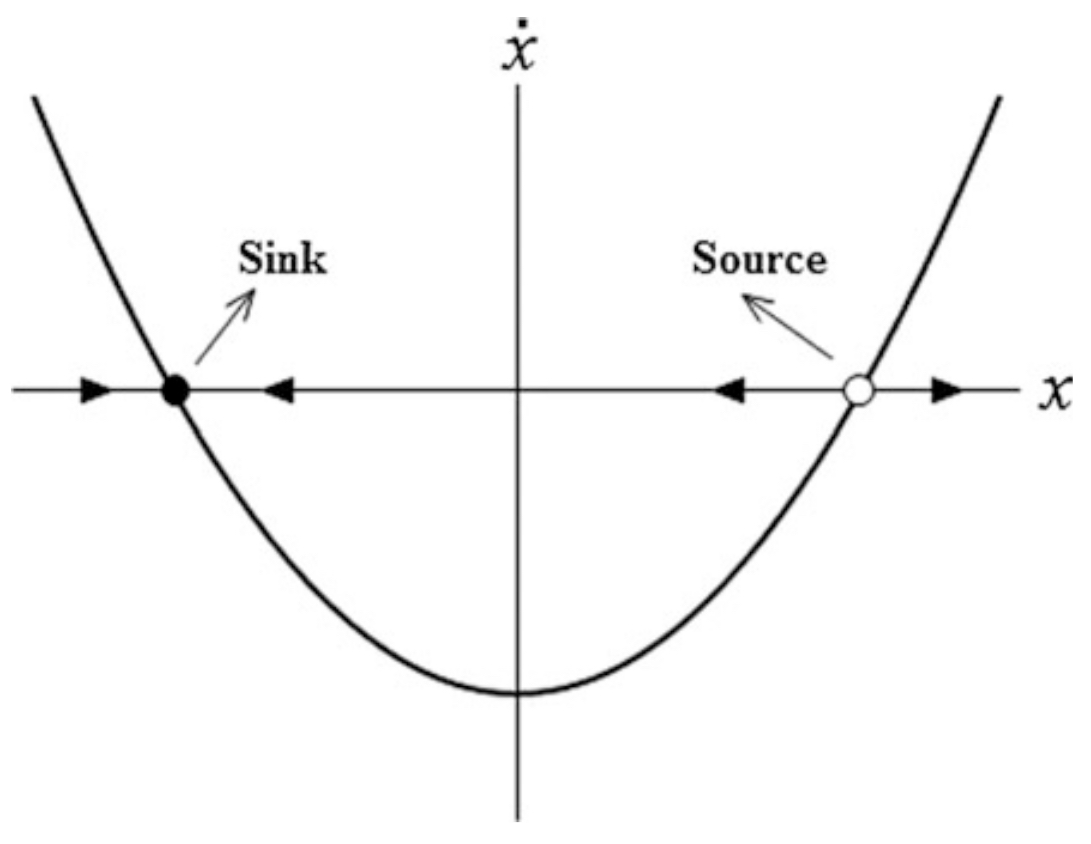
\includegraphics[width=0.4\textwidth]{stability1}
        \caption{Graphical representation of $f(x) = x(1-x)$}
    \end{figure}

\end{frame}


\begin{frame}{Fixed Point Analysis Example 2: Bacteria Growth Model}
    Imagine a small dish where bacteria live.
    \pause{}

    Let $b$ be the relative rate at which the bacteria reproduce.
    \pause{}
    However, the bacteria also produce toxic waste at the rate $px$ (where $x$ is the number of bacteria), which causes them to perish.
    \pause{}

    The number of bacteria increases by $bx$ and their number decreases by $px^{2}$
    \pause{}

    Thus, $\frac{dx}{dt} = bx - px^{2}$.
\end{frame}

\begin{frame}{Bacteria Growth Model Solution}
    To find the fixed point of the system, we need to set the right-hand side of the differential equation to zero.
    \pause{}
    \[b\textsubtilde{x} - p\textsubtilde{x}^{2} = 0\]
    \pause{}
    \[\textsubtilde{x}(b - p\textsubtilde{x}) = 0\]
    \pause{}

    Thus we can see that there are two fixed points:
    \[\textsubtilde{x}_0 = 0 \text{ is \textbf{stable},}\]
    \[\textsubtilde{x}_1 = \frac{b}{p} \text{ is \textbf{unstable}.}\]
\end{frame}

\begin{frame}{Bacteria Growth Model Solution Graph}
    \begin{figure}[t]
        \centering
        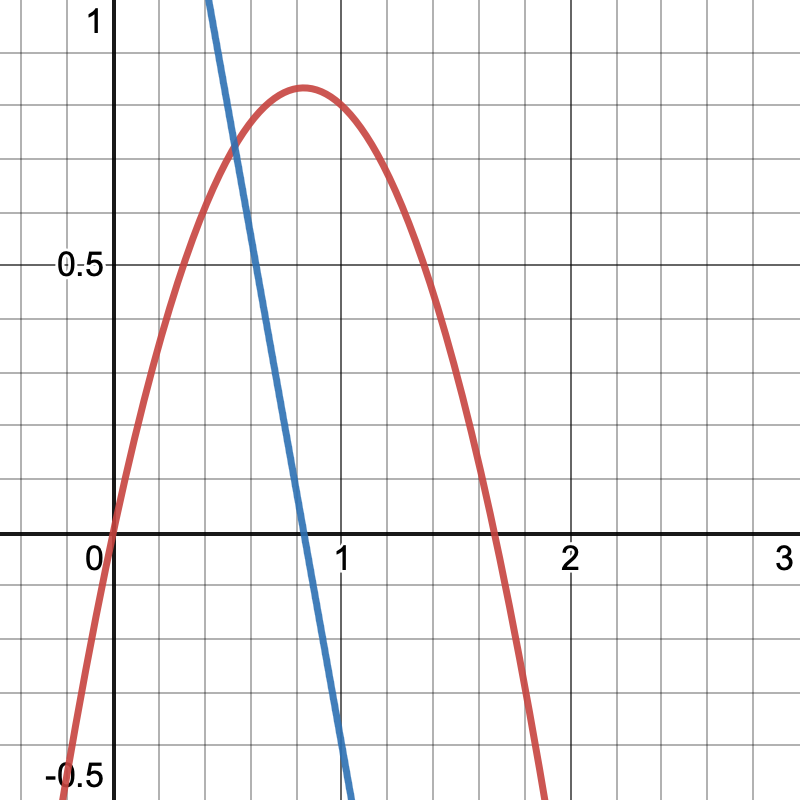
\includegraphics[width=0.5\textwidth]{bacteria-growth-model}
        \caption{Bacteria Growth Model ($b = 2 , p = 1.2$)}
    \end{figure}
\end{frame}

\begin{frame}{Fixed Point Analysis Example 3}
    Consider the following system:
    \[f(x) = \dot{x} = x + x^{3}\]
    \pause{}
    \[f(x) = \dot{x} = x + x^{3} = 0 \implies{x = 0}\]
    \pause{}

    We can see that when $x > 0$, $\dot{x} > 0$ and when $x < 0$, $\dot{x} < 0$. Therefore, the fixed point $x = 0$ is unstable.

    \begin{figure}[t]
        \centering
        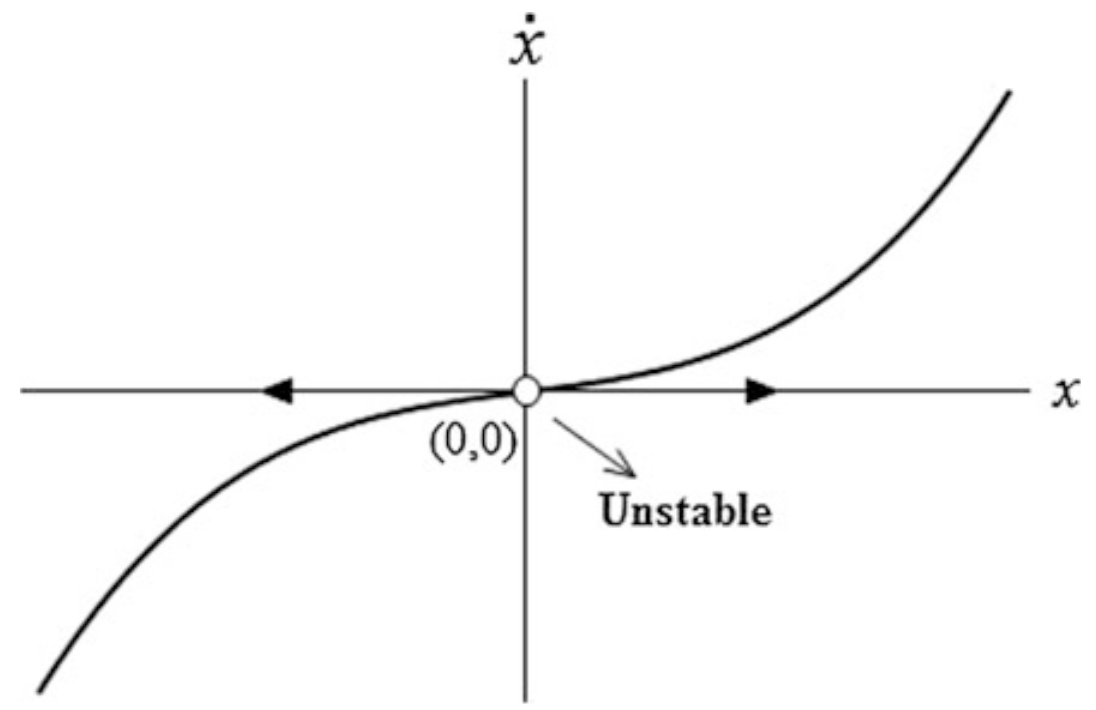
\includegraphics[width=0.3\textwidth]{stability2}
        \caption{Graphical representation of $f(x) = x + x^{3}$}
    \end{figure}
\end{frame}

\begin{frame}{Fixed Point Analysis Example 4}
    Consider the following system:
    \[f(x) = \dot{x} = x - x^{3}\]
    \[f(x) = \dot{x} = x - x^{3} = 0 \implies{x = 0 \text{, } 1 \text{ or } -1}\]
    \pause{}
    We can see that when $x < -1$, $\dot{x} > 0$. When $-1 < x < 0$, $\dot{x} < 0$. When $0 < x < 1$, $\dot{x} > 0$. When $x > 1$, $\dot{x} < 0$.
    \begin{figure}[t]
        \centering
        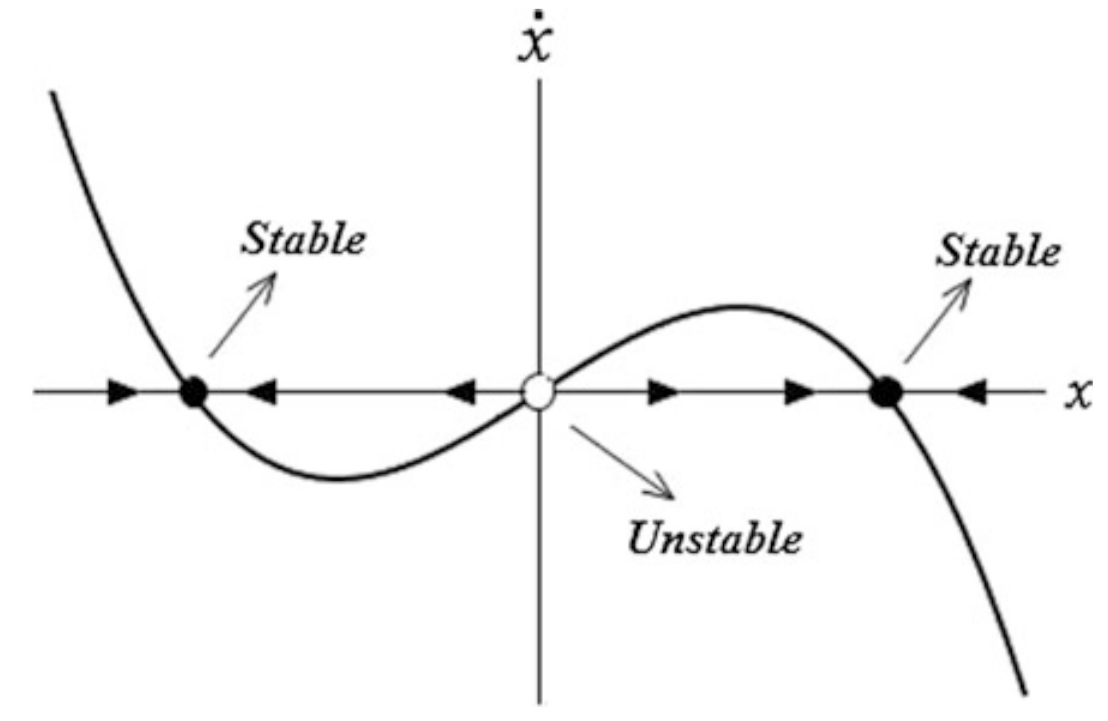
\includegraphics[width=0.4\textwidth]{stability3}
        \caption{Graphical representation of $f(x) = x - x^{3}$}
    \end{figure}
\end{frame}

\begin{frame}{Summary}
    In this presentation, we have 
    \begin{itemize}
        \item defined the concept of \textit{continous dynamical} system;
        \pause{}
    \item presented the types of dynamical systems (\textit{linear} vs \textit{non-linear} and \textit{autonomous} vs \textit{non-autonomous});
        \pause{}
    \item defined the notions of a \textit{flow}, \textit{phase planes and portraits}, as well as the concept of \textit{evolution operator};
        \pause{}
    \item presented the definitions of \textit{fixed points}, classified them into \textit{stable} and \textit{unstable} fixed points, and showed how to identify the type of fixed point;
        \pause{}
        \item covered several illustrative examples for above listed concepts.
    \end{itemize}
\end{frame}

\begin{frame}{Work Cited}
    \begin{thebibliography}{1}
        \bibitem{1}
            \emph{G.C. Layek,}
            \emph{An Introduction to Dynamical Systems and Chaos,}
            \emph{Springer,}
            \emph{2015.}
            \bibitem{2}
                \emph{R. Devaney and L. Devaney,}
                \emph{An Intrduction To Chaotic Dynamical Systems,}
                \emph{Second Edition,}
                \emph{Avalon Publishing,}
                \emph{1989.}
    \end{thebibliography} 
\end{frame}

\begin{frame}
    \thispagestyle{empty}
    \begin{figure}[t]
        \centering
        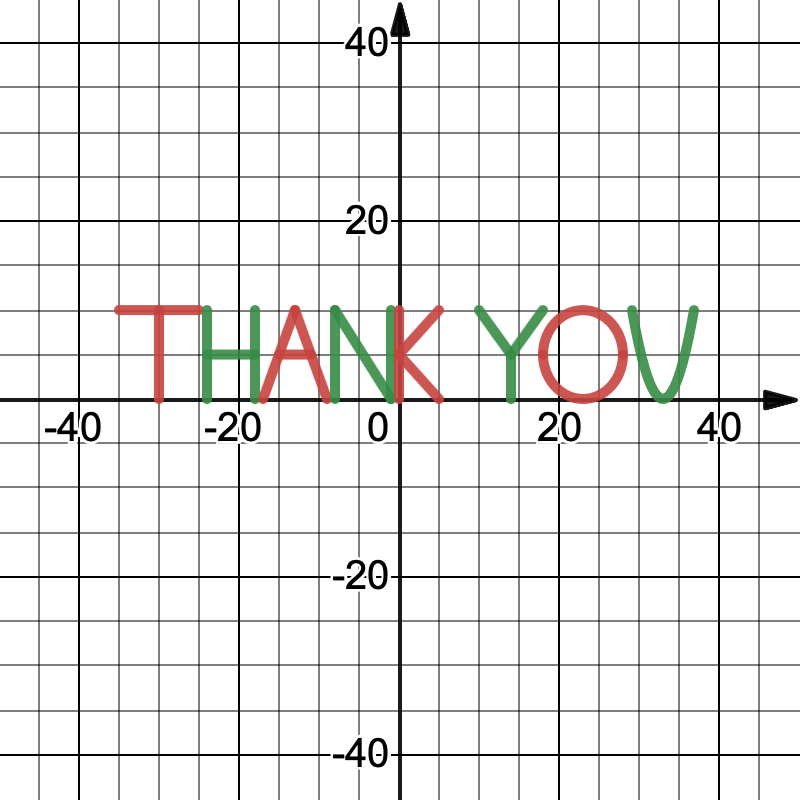
\includegraphics[width=1\textwidth]{thankyou}
    \end{figure}
\end{frame}
\end{document}
